\documentclass[oneside]{book}
\usepackage{glossaries}
\usepackage{derivative}
\usepackage{subcaption}
\usepackage{pgfplots}
\usepackage{graphicx}
\usepackage{tikz}
\usepackage{float}
\usepackage{lipsum}
\usepackage{circuitikz}
\usepackage{amsmath}
\usepackage{amssymb}
\usepackage{caption}
\usepackage{fancyhdr}
\usepackage{enumitem}
\usepackage{lastpage}
\DeclareMathOperator{\sinc}{sinc}
\usepackage[a4paper,
    left=10mm,
    right=10mm,
    top=12mm,
    bottom=12mm,
]{geometry}
\begin{document}
\pagestyle{fancy}
    \fancyhf{}
\fancyhead[L]{EGB242 - Signal Analysis}
\fancyhead[R]{\nouppercase{\leftmark}}
\fancyfoot[L]{Dinal Atapattu}
\renewcommand{\footrulewidth}{0.4pt}
\fancyfoot[R]{Page \thepage\ of \pageref{LastPage}}
    \title{
            Queensland University of Technology\\
            \rule{\linewidth}{0.5pt}
        \centering
        \textbf{EGB242} \\
        Signal Analysis\\
        \vspace{0.4cm}
        \rule{\linewidth}{1.5pt}
        \small{\textit{Profressor Wageeh Boles}}
    }
    \author{Dinal Atapattu}
    \date{\today}
    \maketitle
    \thispagestyle{empty}
    \tableofcontents
    \chapter{Signal Sampling and Quantisation}
        \section{Continuous and Discrete Time Representations}
            \begin{itemize}
                \item An analogue signal is continuous in time and amplitude
                \item A discrete-time signal is discrete in time but continuous in amplitude/value
                \item A digital signal is discrete in time and amplitude
            \end{itemize}
        \section{The Impulse Function}
            The Dirac Delta function $\delta(t)$, is intuitively
            \begin{itemize}
                \item The limit of a pulse of fixed area as its width tends to zero
                \item Area is equal to one
                \item Also called the impulse function
            \end{itemize}
            \begin{minipage}{0.5\linewidth}
                \begin{figure}[H]
                    \centering
                    \begin{tikzpicture}
                        % Draw horizontal axis
                        \draw[-latex] (-3,0) -- (3,0) node[below] {$t$};
                        % Draw vertical axis
                        \draw[-latex] (0,-1) -- (0,3) node[left] {$\delta(t)$};
                      
                        % Draw a red vertical line at x=0
                        \draw[red, thick, -latex] (0,0) -- (0,3);
                      \end{tikzpicture}
                    \caption{Impulse Function}
                    \label{fig:impulse_function}
                \end{figure}
            \end{minipage}
            \begin{minipage}{0.5\linewidth}
                \begin{align*}
                    \delta (t) = 0 && t\neq 0\\
                    \delta (t) \rightarrow \infty && t=0\\
                    \int_{-\infty}^{\infty} \delta (t) dt = 1
                \end{align*}
            \end{minipage}
        \section{Sifting Property of the Impulse}
            \begin{align*}
                \int^{\infty}_{-\infty} f(t)\delta(t-t_0)dt = f(t_0) \tag{$f(t)$ is continuous}
            \end{align*}
            This follows as the impulse function is zero everywhere except at $t=t_0$. So if $t_0 = T_s$ where
            $T_s$ is the sampling interval, then:
            \begin{align*}
                \int_{\infty}^{-\infty} f(t)\delta(t-nT_s)dt = f(nT_s)
            \end{align*}
            Produces the signals at the following intervals/samples $f(0), f(T_s), f(2T_s), f(3T_s), \dots f(nT_s)$
        \section{Analogue to Digital Conversion}
            Consists of 2 steps
                \begin{itemize}
                    \item Sampling
                    \item Quantisation
                \end{itemize}
            \begin{figure}[H]
                \centering
                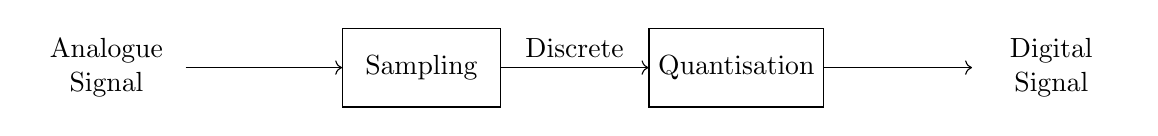
\begin{tikzpicture}
                    \node at (0,0) [minimum width=2cm, minimum height=1cm, align=center] (analogue signal) {Analogue\\Signal};
                    \node at (4,0) [draw, rectangle, minimum width=2cm, minimum height=1cm, align=center] (Sampling) {Sampling};
                    \node at (8,0) [draw, rectangle, minimum width=2cm, minimum height=1cm, align=center] (Quantisation) {Quantisation};
                    \node at (12,0) [minimum width=2cm, minimum height=1cm, align=center] (Digital Signal) {Digital\\Signal};
                    \draw [->] (analogue signal) -- (Sampling);
                    % draw arrow from sampling to quantisation say discrete on top
                    \draw [->] (Sampling) -- (Quantisation) node[midway, above] {Discrete};
                    \draw [->] (Quantisation) -- (Digital Signal);
                \end{tikzpicture}
                \caption{Analogue to Digital Conversion}
                \label{fig:adc}
            \end{figure}
        \section{Sampling Theory}
                A continuous signal with a maximum frequency of $f_m$ can be recovered 
                back grom its samples if the sampling frequency $f_s$ is greater than
                twice the maximum frequency of the continuous signal.\\
                That is $f_s > 2f_m$\\
            \begin{minipage}{0.45\linewidth}
                \centering
                \scalebox{0.8}{
                    \begin{tikzpicture}
                        \begin{axis}[
                            xlabel = $t$,
                            ylabel = {$f(t)$},
                            xmin=-pi, xmax=pi,
                            ymin=-1, ymax=1,
                            % no x or y ticks
                            xtick=\empty, ytick=\empty,
                            % 0 x axis line in the middle
                            axis x line=middle,
                            % remove lines on the side
                            axis y line=middle,
                        ]
                        % plot the sine wave
                        \addplot [
                            domain=-pi:pi, 
                            samples=100, 
                            color=red,
                        ]
                        {-sin(deg(x))};
                        \end{axis}
                    \end{tikzpicture}
                }
                \captionof{figure}{Continuous Signal}
            \end{minipage}
            \begin{minipage}{0.45\linewidth}
                \centering
                \scalebox{0.8}{
                    \begin{tikzpicture}
                        % impulse response of a time domain sine wave
                        \begin{axis}[
                            xlabel = $t$,
                            ylabel = {$\delta(t)$},
                            xmin=-pi, xmax=pi,
                            ymin=-1, ymax=1,
                            % x tick for nT_s
                            xtick={-3.14, -1.57, 0, 1.57, 3.14},
                            xticklabels={$-2T_s$, $-T_s$, $0$, $T_s$, $2T_s$},
                            % no y ticks
                            ytick=\empty,
                            % 0 x axis line in the middle
                            axis x line=middle,
                            % remove lines on the side
                            axis y line=middle,
                        ]
                        % plot the impulses at T_s, 2T_s, 3T_s, 4T_s, straight line going up
                        \foreach \x in {-3,-2,-1,0,1,2,3}
                            \addplot [ycomb, mark=*, color=blue] coordinates {(\x*pi/2, 0.5)};
                        \end{axis}
                    \end{tikzpicture}
                }
                \captionof{figure}{Sampling}
            \end{minipage}
        \section{From Pulse Train to Impulse Train}
            When evaluating the Fourier series of a pulse train with height A, width $\tau$ (area $A\tau$), and period $T_s$
            \begin{equation*}
                c_n = \frac{A\tau}{T_s} \frac{\sin(\pi nf_s \tau)}{\pi n f_s \tau}
            \end{equation*}
            Taking the limit of $\tau \rightarrow 0$:
            \begin{equation*}
                \lim_{\tau \rightarrow 0} \frac{\sin(\pi nf_s \tau)}{\pi n f_s \tau} = \frac{1}{T_s} \lim_{\tau \rightarrow 0} \frac{\sin(\pi nf_s \tau)}{\pi n f_s \tau} = \frac{1}{T_s}
            \end{equation*}
            \begin{align*}
                \delta(t)_{train} &= \sum^{\infty}_{n=-\infty} \frac{1}{T_s} e^{j2\pi nf_s t}\\
                &= \frac{1}{T_s} + \sum_{\substack{n=-\infty\\ n\neq 0}}^{\infty} \frac{2}{T_s}\cos\left(2\pi n f_s t\right)
            \end{align*}
        \section{Sampling Process}
            Sampling of a discrete signal can be obtained by multiplying the signal 
            by an impulse train $\delta(t)$ of period $T_s$. The output of the 
            multiplier is a discrete signal called the sample signal\\
            The spectra of the input and sampled signals are represented as
            \begin{figure}[H]
                \begin{subfigure}{0.5\textwidth}
                    \centering
                    \begin{tikzpicture}
                        \begin{axis}[
                            xlabel = $t$,
                            ylabel = {$X(\omega)$},
                            xmin=-3, xmax=3,
                            ymin=-2, ymax=2,
                            % x tick for nT_s
                            xtick=\empty,
                            % no y ticks
                            ytick=\empty,
                            % 0 x axis line in the middle
                            axis x line=middle,
                            % remove lines on the side
                            axis y line=middle,
                        ]
                        \addplot [
                            domain=-1:0, 
                            samples=100, 
                            color=red,
                        ] {x + 1};
                        \addplot [
                            domain=0:1, 
                            samples=100, 
                            color=red,
                        ] {-x + 1};
                        \end{axis}
                    \end{tikzpicture}
                \end{subfigure}
                \begin{subfigure}{0.5\textwidth}
                    \begin{tikzpicture}
                        \begin{axis}[
                            xlabel = $t$,
                            ylabel = {$Y(\omega)$},
                            xmin=-12, xmax=12,
                            ymin=-8, ymax=8,
                            xtick={-6, 0, 6},
                            xticklabels={$-\omega_s$, $0$, $\omega_s$},
                            ytick=\empty,
                            axis x line=middle,
                            axis y line=middle,
                        ]
                        \addplot [
                            domain=-3:0, 
                            samples=100, 
                            color=red,
                        ] {x + 3*1};
                        \addplot [
                            domain=3:6, 
                            samples=100, 
                            color=red,
                        ] {x - 3};
                        \addplot [
                            domain=-9:-6, 
                            samples=100, 
                            color=red,
                        ] {x + 3*3};
                        \addplot [
                            domain=6:9, 
                            samples=100, 
                            color=red,
                        ] {-x + 3*3};
                        \addplot [
                            domain=-6:-3,
                            samples=100, 
                            color=red,
                        ] {-x - 3};
                        \addplot [
                            domain=0:3, 
                            samples=100, 
                            color=red,
                        ] {-x + 3*1};
                        \end{axis}
                    \end{tikzpicture}
                \end{subfigure}
            \end{figure}
        \section{Anti-Aliasing}
            Hardware constraints may not allow sampling at the Nyquist frequency.\\
            By using an anti-aliasing (low-pass) filter before the sampling stage, we can eliminate spectral overlap.\\
            This lowpass filter must have a bandwidth at or below $\frac{f_s}{2}$\\
            Example: If an analog signal has a bandwidth of 2 kHz and must be sampled at 3 kHz, then the anti-aliasing filter must have a bandwidth of 1 kHz or less.
            \begin{figure}[H]
                \centering
                \includegraphics[width=0.5\linewidth]{figures/aa_spectra.png}
                \caption{Anti-Aliasing Spectra}
            \end{figure}
        \section{Anti-Aliasing Spectrum}
            \begin{figure}[H]
                \centering
                \includegraphics[width=0.5\linewidth]{figures/aa_spectrum.png}
                \caption{Anti-Aliasing Spectrum}
            \end{figure}
        \section{Discrete to Digital}
            Digital signals are discrete in time AND amplitude. The quantizer 
            transforms each sampled value to take one of $L$ distinct levels.
            \begin{figure}[H]
                \centering
                \includegraphics[width=0.5\linewidth]{figures/quantiser.png}
                \caption{Quantiser}
            \end{figure}
            These leves are allocated over the entire dynamic range of the analog
            signal.
            \begin{equation*}
                x_{\text{min}} \leq x(t) \leq x_{\text{max}}
            \end{equation*}
            This is lossy and non-invertible.
            \subsection{Uniform Quantiser}
                Levels are \textbf{uniformly} allocated across the dynamic range\\
                The step size $\Delta$ between quantization levels is given by
                \begin{equation*}
                    \Delta = \frac{x_{\text{max}} - x_{\text{min}}}{L}
                \end{equation*}
                Many applications have $x_{\text{max}} = -x_{\text{min}}$. Which gives
                \begin{equation*}
                    \Delta = \frac{2x_{\text{max}}}{L}
                \end{equation*}
                The number of levels is often chosen to be a power of two to better
                use binary words
                \begin{equation*}
                    L = 2^n
                \end{equation*}
                Where $n$ is the number of bits used to encode $L$ levels.
                \subsubsection{Example}
                    A signal with a dynamic range between $\pm 4V$ is to be uniformly quantiszed with each level encoded by 4 bits.\\
                    What is the step size between bits.
                    \begin{itemize}
                        \item $n = 4 \text{ bits}$
                        \item $L = 2^n = 2^4 = 16 \text{ levels}$
                        \begin{equation*}
                            \Delta = \frac{2x_{\text{max}}}{L} = \frac{2(4)}{16} = 0.5V
                        \end{equation*}
                        \item 4 bits allow for encoding 16 unique code words
                        \item Each code word represents a single quantization level
                    \end{itemize}
            \subsubsection{Uniform Quantizer Types}
                \begin{itemize}[label=--]
                    \item \textbf{Mid-tread} quantizer\\
                    \begin{minipage}[t]{0.35\linewidth}
                        \includegraphics[width=\textwidth]{figures/mid_riser_transfer_function.png}
                    \end{minipage}
                    \begin{minipage}[t]{0.45\linewidth}
                        \begin{itemize}
                            \item Enforces a quantisation step at zero
                            \item $L$ is odd if $x_{\text{min}} = -x_{\text{max}}$
                            \item May waste one level
                        \end{itemize}
                    \end{minipage}
                    \item \textbf{Mid-rise} quantizer\\
                    \begin{minipage}[t]{0.35\linewidth}
                        \includegraphics[width=\textwidth]{figures/mid_tread_transfer_function.png}
                    \end{minipage}
                    \begin{minipage}[t]{0.45\linewidth}
                        \begin{itemize}
                            \item $L$ levels are evenly distributed about 0
                            \item Can't guarantee 0
                            \item Uses all levels when $x_{\text{min}} = -x_{\text{max}}$
                        \end{itemize}
                    \end{minipage}
                \end{itemize}
            \subsection{Quantisation Error}
                Quantisation error is the difference between the quantised signal and the sampled signal
                \begin{equation*}
                    e_q(n) = x(n) - \hat{x}(n)
                \end{equation*}
                This is a function of $n$, where $n$ is the sample number.\\
            \subsection{Signal to Quantisation Noise Ratio}
                SQNR represents the amount of distortion due to quantisation defined as the ratio of
                signal power to the quantisation noise power
                \begin{equation*}
                    \text{SQNR} = \frac{\text{Signal Power}}{\text{Quantisation Noise Power}}
                \end{equation*}
                The difference between the sampled signal and quantised signal is the quantisation error.
            \subsection{Quantisation Noise Power}
                Quantisation noise power is the variance of the quantisation error\\
                Can be treated as a uniformly distruibuted random variable between $\frac{\Delta}{2}$ and $\frac{\Delta}{2}$\\
                \begin{equation}
                    \text{P}_{\text{noise}} = \int^{\infty}_{-\infty} e^2 f(e) de = \frac{\Delta}{12}
                \end{equation}
            \subsection{Noise Power as a Function of n}
                Expressing the noise power as a function of n gives
                    \begin{align}
                        \text{P}_{\text{noise}} &= \frac{\Delta^2}{12} = \frac{1}{12} \times \left(\frac{x_{\text{max}} - x_{\text{min}}}{L}\right)^2 \notag\\
                        &= \frac{x_{\text{max}}^2 - x_{\text{min}}^2}{12 n^2}
                    \end{align}
                Increasing the number of quantisation levels improves SQNR. The number of representation levels is determined by
                the number of bits used to encode the sample $L=2^n$. PCM for example encodes each sample with equal length binary words.
            \subsection{Limitations}
                While qunatisation noise power is equal across the input signal range, the input signal's power changes across decision levels.
                Resulting in differing SQNR across the input signal range.\\
                For example with human speech, louder sounds carry higher signal power than softer sounds.\\
                Uniform quantisation would result in different SQNR for different sounds.\\
            \subsection{Non-Uniform Quantisers}
                A constant SQNR can be achieved using a non uniform quantiser. These have different step sizes over their dynamic range, allocating more levels
                to the range of signals with smaller power.
                \begin{figure}[H]
                    \centering
                    \includegraphics[width=0.4\linewidth]{figures/non_uniform_quantiser.png}
                    \caption{$\mu$ Law Non-Uniform Quantiser Transfer Function}
                \end{figure}
        \section{Encoding}
            \subsection{Waveform Encoding}
                Encodes each quantized sample as a string of bits
                \begin{itemize}
                    \item Pulse Code Modulation (PCM)
                    \item Differential Pulse Code Modulation (DPCM)
                    \item Shannon-Fano Encoding
                    \item Huffman Encoding
                \end{itemize}
                \subsubsection{Pulse Code Modulation}
                    Each sample is an equal length code binary word with length n bits, allowing for $2^n$ encoding levels and
                    is the standard for analogue to digital (A/D) conversion.
    \chapter{Linear Time Invariant Systems}
        \section{Transfer Functions}
            \begin{itemize}
                \item Time domain output $\longrightarrow$ convolution of time domain input with impulse response of the system
                    \subitem $y(t) = x(t) * h(t)$
                \item Spectrum of the output $\longrightarrow$ product of the Fourier transform of the input with the Fourier transform of the impulse response
                    \subitem $Y(f) = X(f)H(f)$
                \item Fourier Transform of the impulse response $\longrightarrow$ Transfer Function
                    \subitem $H(f) = \frac{Y(f)}{X(f)}$
                    \subitem Provides the system's gain and phase change information
            \end{itemize}
        \section{Transfer Functions from Block Diagrams}
            \begin{figure}[H]
                \centering
                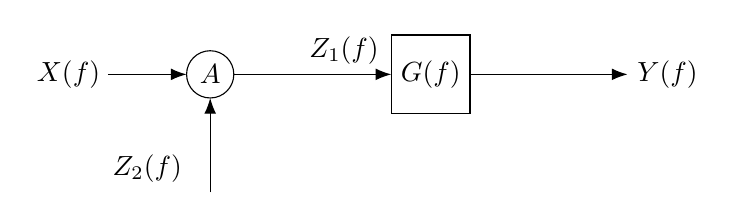
\begin{tikzpicture}
                    \node at (0,0) {$X(f)$};
                    \draw[-{Latex[length=2mm]}] (0.5,0) -- (1.5,0);
                    \draw (1.8,0) circle (0.3);
                    \node at (1.8,0) {$A$};
                    \draw[-{Latex[length=2mm]}] (2.1,0) -- (4.1,0);
                    \draw (4.1,-0.5) rectangle (5.1,0.5) node[pos=.5, align=center] {$G(f)$};
                    \draw[-{Latex[length=2mm]}] (5.1,0) -- (7.1,0) node[pos=1, right] {$Y(f)$};
                    \draw[-{Latex[length=2mm]}] (1.8,-1.5) -- (1.8,-0.3);
                    \node at (1,-1.2) {$Z_2(f)$};
                    \node at (3.5,0.3) {$Z_1(f)$};
                \end{tikzpicture}
            \end{figure}
            \begin{flalign*}
                \intertext{From the block diagram we can see that:}
                Z_1(f) &= X(f) - Z_2(f) \tag{1}\\
                Z_2(f) &= k Y(f) \tag{2}\\
                \intertext{Substituting (2) into (1) gives:}
                Z_1(f) &= X(f) - kY(f)\\
                \intertext{Note that:}
                Y(f) &= G(f)X(f) \tag{3}
                \intertext{Substituting this into the above equation gives:}
                Y(f) &= G(f)\left(X(f) - kY(f)\right)\\
                &= G(f)X(f) - kG(f)Y(f) \tag{4}\\
                \intertext{Therefore:}
                Y(f) + kG(f)Y(f) &= G(f)X(f)\\
                Y(f)\left(1 + kG(f)\right) &= G(f)X(f)\\
                \frac{Y(f)}{X(f)} &= \frac{G(f)}{1 + kG(f)} \tag{5}\\
            \end{flalign*}
        \section{Filters}
            Attenuate certain ranges of frequencies in a signal
            In the following forms
            \begin{itemize}
                \item Lowpass
                    \subitem Only allows low frequencies to pass
                \item Highpass
                    \subitem Only allows high frequencies to pass
                \item Bandpass
                    \subitem Only allows a band of frequencies to pass
                \item Bandstop
                    \subitem Only blocks a band of frequencies
            \end{itemize}
            Note that:
            \begin{itemize}
                \item \textcolor{red}{Pass band} is the range of frequencies that are allowed to pass
                \item \textcolor{red}{Stop band} is the range of frequencies that are blocked
            \end{itemize}
            \subsection{Ideal Filters}
                They are unrealisable (cannot exist in the real world) and have the following characteristics
                \begin{itemize}
                    \item Completely attenuate signals in their stop bands
                    \item Completely pass signals in their pass bands
                    \item Immediately transition between pass and stop bands
                    \item Have no effect on phase
                \end{itemize}
            \subsection{Practical Filters}
                \begin{figure}[H]
                    \centering
                    \includegraphics[width=0.5\linewidth]{figures/practical_filter.png}
                    \caption{Ideal Filter}
                \end{figure}
        \chapter{Fourier Transform}
            \section{Euler's Identity}
                \begin{align*}
                    \cos(\theta) = \frac{e^{j\theta} + e^{-j\theta}}{2}\\   
                    \sin(\theta) = \frac{e^{j\theta} - e^{-j\theta}}{2j}
                \end{align*}
            \section{Exponential Fourier Series}
                \begin{align*}
                    s(t) = \sum^{\infty}_{n=-\infty} c_n e^{j2\pi n f_0 t}\\
                    c_n = \frac{1}{T} \int^{T}_{0} s(t) e^{-j2\pi n f_0 t} dt
                \end{align*}
                Multiplying by $e^{-j2\pi m f_0 t}$ and integrating over one period removes all
                frequency excepts those at $nf_0$.
            \section{Transforms}
                \subsection{Fourier Transform}
                    \begin{align*}
                        G(f) &= \int^{\infty}_{-\infty} g(t) e^{-j2\pi f t} dt\\
                    \end{align*}
                \subsection{Inverse Fourier Transform}
                    \begin{align*}
                        g(t) &= \int^{\infty}_{-\infty} G(f) e^{j2\pi f t} df\\
                    \end{align*}
            \section{Linearity}
                \begin{figure}[H]
                    \centering
                    \includegraphics[width=0.5\linewidth]{figures/linearity.png}
                    \caption{Sawtooth Wave}
                \end{figure}
                \begin{align*}
                    c_n &= \frac{1}{T} \int^{T}_{0} s(t) e^{-j2\pi n f_0 t} dt, f_0  \frac{1}{T}\\
                    &= \frac{1}{T} \left(\int^{\frac{T}{2}}_{0} t e^{-j2\pi n t} dt - \int^{T}_{\frac{T}{2}} t e^{-j2\pi n t} dt\right)\\
                    &= \frac{1}{T} \left(\int^{\frac{T}{2}}_{0} t e^{-j2\pi n \frac{1}{T} t} dt - \int^{T}_{\frac{T}{2}} t e^{-j2\pi n \frac{1}{T} t} dt\right)\\
                \end{align*}
            \section{Alternate Expression of the Fourier Series}
                \begin{align*}
                    c_0 &= \frac{1}{T} \int^{T}_{0} s(t) dt\\
                    c_n &= \frac{1}{T} \int^{T}_{0} s(t) e^{-j2\pi n f_0 t} dt\\
                    s(t) &= c_0 + \sum_{\substack{n=-\infty\\ n\neq 0}}^{\infty} c_n e^{j2\pi n f_0 t}\\
                \end{align*}
                In this form, $c_0$ is the DC component of the signal and $c_n$ is the amplitude of the $n$th harmonic.
            \section{Gate Function}
                \begin{figure}[H]
                    \centering
                    \includegraphics[width=0.5\linewidth]{figures/gate.png}
                    \caption{Gate Function}
                \end{figure}
                \begin{flalign*}
                    \Pi_T \left(t\right)\\
                    rect \left(\frac{t}{T}\right)\\
                \end{flalign*}
                \subsection{Fourier Transform}
                    \begin{flalign*}
                        \mathcal{F}\left\{ \Pi_T\left(t\right) \right\} &= \int^{\infty}_{-\infty} \Pi_T\left(t\right) e^{-j2\pi f t} dt\\
                        &= \int^{\frac{T}{2}}_{-\frac{T}{2}} e^{-j2\pi f t} dt\\
                        &= \frac{1}{-j2\pi f} \left[e^{-j2\pi f t}\right]^{\frac{T}{2}}_{-\frac{T}{2}}\\
                        &= \frac{1}{-j2\pi f} \left[e^{-j2\pi f \frac{T}{2}} - e^{j2\pi f \frac{T}{2}}\right]\\
                        &= \frac{1}{-j2\pi f} \left[e^{-j\pi f T} - e^{j\pi f T}\right]\\
                        &= \frac{1}{\pi f} \left[\frac{e^{j\pi f T} - e^{-j\pi f T}}{2j}\right]\\
                        &= \frac{T}{T\pi f} \left[\frac{e^{j\pi f T} - e^{-j\pi f T}}{2j}\right]\\
                        &= T\sinc(Tf)\\
                    \end{flalign*}
                \subsection{Time Shifted Gate Function}
                    \begin{figure}[H]
                        \centering
                        \includegraphics[width=0.5\linewidth]{figures/gate_timeshift.png}
                        \caption{Time-Shifted Gate Function}
                    \end{figure}
                    \begin{flalign*}
                        \mathcal{F}\left\{ \Pi_T\left(t\right) \right\} &= \int^{\infty}_{-\infty} \Pi_T\left(t\right) e^{-j2\pi f t} dt\\
                        &= \int^{\frac{t_0 + T}{2}}_{t_0 -\frac{T}{2}} e^{-j2\pi f t} dt\\
                        &= \frac{1}{-j2\pi f} \left[e^{-j2\pi f t}\right]^{\frac{t_0 + T}{2}}_{t_0 -\frac{T}{2}}\\
                        &= \frac{1}{-j2\pi f} \left[e^{-j2\pi f \frac{t_0 + T}{2}} - e^{j2\pi f \frac{t_0 + T}{2}}\right]\\
                        &= \frac{e^{-2j\pi ft_0}}{\pi f} \left[\frac{e^{j\pi f T} - e^{-j\pi f T}}{2j}\right]\\
                        &= \frac{e^{-2j\pi ft_0}}{\pi f} \left[\frac{T\left(e^{j\pi f T} - e^{-j\pi f T}\right)}{2Tj}\right]\\
                        &= e^{-j2\pi ft_0}T\sinc\left(fT\right)
                    \end{flalign*}
        \chapter{Laplace Transform}
            \section{Relationship with the Fourier Transform}
                \begin{align*}
                    G(s) &= \int^{\infty}_{-\infty} g(t) e^{-\left(\sigma + j\omega t \right)} dt\\
                    &= \int^{\infty}_{-\infty} g(t) e^{-\sigma t} e^{-j\omega t} dt\\
                    \intertext{Where $\sigma$ is the real part of $s$ and $\omega$ is the imaginary part of $s$}
                    \intertext{for $\sigma = 0$}
                    G(j\omega) &= \int^{\infty}_{-\infty} g(t) e^{-j\omega t} dt\\
                    G(j\omega) &= \int^{\infty}_{-\infty} g(t) e^{-j2\pi n ft} dt = G(f)\\
                \end{align*}
            \section{Region of Convergence (ROC)}
                The Laplace Transform exists for all complex numbers if $a < Re\{s\} < b$ where $a$ and $b$ are real numbers.\\
                The set of values of $s$ for which the Laplace Transform converges is called the Region of Convergence (ROC).\\
            \section{Circuit Analysis}
                \begin{figure}[H]
                    \centering
                    \begin{tabular}{|c|c|c|}
                        \hline
                        Element & Time Domain & Laplace Domain \\
                        \hline
                        Resistor & $R$ & $R$ \\
                        \hline
                        Capacitor & $\frac{1}{C} \int i(t) \, dt$ & $\frac{1}{Cs}$ \\
                        \hline
                        Inductor & $L \frac{di(t)}{dt}$ & $Ls$ \\
                        \hline
                    \end{tabular}
                    \caption{Circuit Analysis}
                \end{figure}
                Done in the following steps
                \begin{enumerate}
                    \item Convert circuit components, voltages, and currents to Laplace domain
                    \item Obtain the transfer function in the Laplace domain using mesh, nodal or any other circuit analysis technique (may need
                    to be simplified using Partial Fraction Expansion)
                    \item Convert the transfer function back to the time domain using the inverse Laplace Transform
                \end{enumerate}
            \section{Partial Fraction Expansion}
                \begin{figure}[H]
                    \centering
                    \begin{tabular}{|c|c|}
                        \hline
                        \textbf{Form of the Rational Function} & \textbf{Partial Fraction Expansion}\\
                        \hline
                        $\frac{ps+q}{(s+a)(s+b)}$ & $\frac{A}{s+a} + \frac{B}{s+b}$\\
                        \hline
                        $\frac{ps+q}{(s+a)^2}$ & $\frac{A}{s+a} + \frac{B}{(s+a)^2}$\\
                        \hline
                        $\frac{ps^2+qs+r}{(s+a)(s+b)(s+c)}$ & $\frac{A}{s+a} + \frac{B}{s+b} + \frac{C}{s+c}$\\
                        \hline
                        $\frac{ps^2+qs+r}{(s+a)^2(s+b)}$ & $\frac{A}{s+a} + \frac{B}{(s+a)^2} + \frac{C}{s+b}$\\
                        \hline
                        $\frac{ps^2+qs+r}{(s+a)(s^2+bs+c)}$ & $\frac{A}{s+a} + \frac{Bs+C}{s^2+bs+c}$\\
                        \hline
                    \end{tabular}
                    \caption{Partial Fraction Expansion Forms}
                \end{figure}
                \begin{enumerate}
                    \item Factorise the denominator of the transfer function
                    \item Write the transfer function as a sum of fractions with the factors of the denominator as the denominators of the fractions
                    \item Write the numerator of the transfer function as the numerator of the fractions
                    \item Solve for the unknown coefficients
                    \item Convert the fractions back to the time domain using the inverse Laplace Transform
                \end{enumerate}
                Example:
                \begin{align*}
                    H(s) &= \frac{1}{s^2 + 2s + 1}\\
                    &= \frac{1}{(s+1)^2}\\
                    &= \frac{A}{s+1} + \frac{B}{(s+1)^2}\\
                    &= \frac{A(s+1) + B}{(s+1)^2}\\
                    &= \frac{As + A + B}{(s+1)^2}\\
                    \intertext{Comparing coefficients gives:}
                    A &= 1\\
                    A + B &= 0\\
                    B &= -1\\
                    \intertext{Therefore:}
                    H(s) &= \frac{1}{s+1} - \frac{1}{(s+1)^2}\\
                    &= \frac{1}{s+1} - \frac{1}{s+1} + \frac{1}{(s+1)^2}\\
                    &= \frac{1}{s+1} - \frac{1}{(s+1)^2}\\
                    &= e^{-t} - te^{-t}
                \end{align*}
    \chapter{System Characterisation}
        % table of step responses for different second order systems with plots
        \section{Second Order Systems}
            Systems in the form of
            \begin{equation*}
                \frac{Y(s)}{X(s)} = \frac{\omega_n^2}{s^2 + 2\zeta\omega_n s + \omega_n^2}
            \end{equation*}
            \begin{figure}[H]
                \centering
                \begin{tabular}{|c|c|c|c|c|}
                    \hline
                    \textbf{System Type} & \textbf{Nature of Roots} & \textbf{Condition} & \textbf{Roots} & \textbf{System Figure} \\
                    \hline
                    Overdamped & Two Real Roots & $\zeta > 1$ & $s_1 = -\zeta\omega_n + \omega_n\sqrt{\zeta^2 - 1}$ & 
                    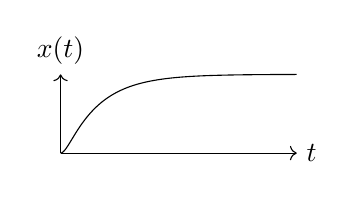
\begin{tikzpicture}[xscale=0.5]
                        \draw[->] (0,0) -- (6,0) node[right] {$t$};
                        \draw[->] (0,0) -- (0,1) node[above] {$x(t)$};
                        \draw[domain=0:6,variable=\t,smooth,samples=200] plot ({\t},{1 + 0.171*exp(-7.854*\t) - 1.171*exp(-1.146*\t)});
                    \end{tikzpicture} \\
                    \hline
                    Critically Damped & One Real Root & $\zeta = 1$ & $s_1 = -\zeta\omega_n$ & 
                    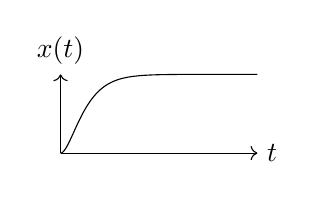
\begin{tikzpicture}[xscale=0.5]
                        \draw[->] (0,0) -- (5,0) node[right] {$t$};
                        \draw[->] (0,0) -- (0,1) node[above] {$x(t)$};
                        \draw[domain=0:5,variable=\t,smooth,samples=200] plot ({\t},{1 - 3*exp(-3*\t)*\t - exp(-3*\t)});
                    \end{tikzpicture} \\
                    \hline
                    Underdamped & Two Complex Roots & $0 < \zeta < 1$ & $s_1 = -\zeta\omega_n \pm j\omega_n\sqrt{\zeta^2 - 1}$ & 
                    \begin{tikzpicture}[xscale=0.5]
                        \draw[->] (0,0) -- (5,0) node[right] {$t$};
                        \draw[->] (0,0) -- (0,1.4) node[above] {$x(t)$};
                        \draw[domain=0:5,variable=\t,smooth,samples=200] plot ({\t},{1-1.06*exp(-1*\t)*cos(deg(sqrt(8)*\t - 19.47))});
                    \end{tikzpicture} \\
                    \hline
                    Undamped & Two Imaginary Roots & $\zeta = 0$ & $s_1 = \pm j\omega_n$ & 
                    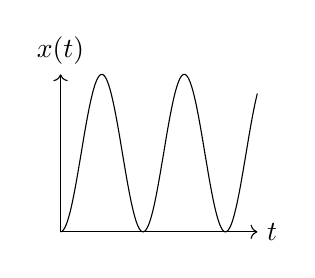
\begin{tikzpicture}[xscale=0.5]
                        \draw[->] (0,0) -- (5,0) node[right] {$t$};
                        \draw[->] (0,0) -- (0,2) node[above] {$x(t)$};
                        \draw[domain=0:5,variable=\t,smooth,samples=200] plot ({\t},{1 - cos(deg(3*\t))});
                    \end{tikzpicture} \\
                    \hline
                \end{tabular}
                \caption{Second Order Systems}
            \end{figure}
            \begin{itemize}
                \item $\omega_n$ is the natural frequency
                \item $\zeta$ is the damping ratio
            \end{itemize}
        \section{Natural Response By Inspection}
            \begin{itemize}
                \item Overdamped, poles at $-\sigma_1, -\sigma_2$
                    \subitem $y(t) = A_1e^{-\sigma_1 t} + A_2e^{-\sigma_2 t}$
                \item Underdamped, poles at $-\sigma \pm j\omega_d$
                    \subitem $y(t) = Ae^{-\sigma t}\cos(\omega_d t + \phi)$
                \item Undamped, poles at $\pm j\omega_n$
                    \subitem $y(t) = A\cos(\omega_n t + \phi)$
                \item Critically damped, poles at $-\sigma$
                    \subitem $y(t) = (A_1 + A_2t)e^{-\sigma t}$
            \end{itemize}
        \section{Poles of general 2nd order systems}
            \begin{equation}
                G(s) = \frac{\omega_n^2}{s^2 + 2\zeta\omega_n s + \omega_n^2}
            \end{equation}
            The roots of the denominator polynomial are the poles of the system
            \begin{equation}
                s^2 + 2\zeta\omega_n s + \omega_n^2 = 0
            \end{equation}
            \begin{equation}
                s_{1,2} = -\zeta\omega_n \pm \omega_n\sqrt{\zeta^2 - 1}
            \end{equation}
        \section{Step Response of Underdamped 2nd Order Systems}
            Specifications are 
            \begin{itemize}
                \item Settling Time
                    \subitem $T_s = \frac{4}{\zeta\omega_n}$
                \item \% Overshoot
                    \subitem $\%OS= e^{\frac{-\zeta\pi}{\sqrt{1 - \zeta^2}}}\times 100$
                \item Peak Time
                    \subitem $T_p = \frac{\pi}{\omega_n \sqrt{1 - \zeta^2}}$
            \end{itemize}
        \section{Step Response of a 1st Order System}
            Specifications are
            \begin{itemize}
                \item Settling Time
                    \subitem $T_s = \frac{4}{\alpha}$
                \item Rising Time
                    \subitem $T_r = \frac{2.2}{\alpha}$
            \end{itemize}
    \chapter{Tutorial Questions}
        \section{Tutorial 13}
            \subsection*{Question 1}
                \begin{figure}[H]
                    \centering
                    \includegraphics[width=\linewidth]{figures/tute13_q1.png}
                \end{figure}
            Express $s_1(t)$ and $s_2(t)$ as complex Fourier series.\\
            \begin{align*}
                s_1(t) = \begin{cases}
                    1 & -\frac{1}{2} \leq t < 0\\
                    -1 & 0 \leq t < \frac{1}{2}\\
                \end{cases}
            \end{align*}
            Note that $T = 1$ and $f_0 = \frac{1}{T} = 1$\\
            \begin{minipage}[t]{0.45\textwidth}
                Part 1:
                \begin{flalign*}
                c_0 &= \int^{\infty}{-\infty} s_1(t) dt\\
                &= \int^{0}{-0.5} 1 dt + \int^{0.5}{0} -1 dt\\
                &= \left[t\right]^{0}{-0.5} + \left[-t\right]^{0.5}{0}\\
                &= 0.5 - 0.5 = 0
                \end{flalign*}
                \end{minipage}
                \hfill
            \begin{minipage}[t]{0.45\textwidth}
                Part 2:
                \begin{flalign*}
                c_n &= \frac{1}{T} \int^{\infty}{-\infty} s_1(t) e^{-j2n\pi f_0 t} dt\\
                &= \frac{1}{1} \int^{0}{-0.5} e^{-j2n\pi t} dt + \frac{1}{1} \int^{0.5}{0} -e^{-j2n\pi t} dt\\
                &= \int^{0}{-0.5} e^{-j2n\pi t} dt + \int^{0}{0.5} e^{-j2n\pi t} dt\\
                &= \left[\frac{e^{-j2n\pi t}}{-j2n\pi}\right]^{0}{-0.5} + \left[\frac{e^{-j2n\pi t}}{-j2n\pi}\right]^{0.5}{0}\\
                &= \frac{e^{-j2n\pi \times 0.5}}{-j2n\pi} - \frac{e^{-j2n\pi \times 0}}{-j2n\pi} + \frac{e^{-j2n\pi \times 0.5}}{-j2n\pi} - \frac{e^{-j2n\pi \times 0}}{-j2n\pi}\\
                &= \frac{e^{-jn\pi}}{-j2n\pi} - \frac{1}{-j2n\pi} + \frac{e^{-jn\pi}}{-j2n\pi} - \frac{1}{-j2n\pi}\\
                &= \frac{e^{-jn\pi}}{-jn\pi} - \frac{1}{-jn\pi}\\
                &= \frac{j}{\pi n} \left(\left(-1\right)^n - 1\right)\\
                \end{flalign*}
            \end{minipage}\\
            Therefore:
            \begin{equation*}
                s_1(t) = \sum^{\infty}_{n=-\infty} \frac{j}{\pi n} \left(\left(-1\right)^n - 1\right) e^{j2n\pi t}\\
            \end{equation*}
\end{document}